\section{Exercise 2}
In this exercise, we interpolate through points from a Vandermonde matrix using LU Decomposition (LUD) and Neville's Algorithm. We start by importing the data from the Vandermonde matrix and iterating through the rows and columns to create a matrix object using that $V_{ij} = x^i_{j}$. 

\subsection{2A}
We opted to use the improved version of Crout's algorithm for LUD for better stability and performance. For this, we attempted to, as closely as possible, resemble the steps described in Lecture 3, slide 15 in the code. With the LUD matrix created, we performed forward and backward substitution. Here, we mostly used the equations from Lecture 3, slide 11. In the forward substitution, we set $\alpha_{ii} = 1$, so this variable does not appear in the code. Moreover, we noticed that two backward loops were necessary to have the backward substitution function properly, which was not immediately obvious from the equation. From this, we obtained the values of \textbf{c}, which we show below in the text output. Using Eq. 2 of the Hand-in, we iterated both through the original sample points and the 1000 values we wished to interpolate to compute the 19th-degree polynomial. The interpolated polynomial goes through all sample points, with expected oscillation nearing the end (as this is close to a Lagrange polynomial), see Figure \ref{fig:2A_interp}. 

\begin{figure}[h!]
  \centering
  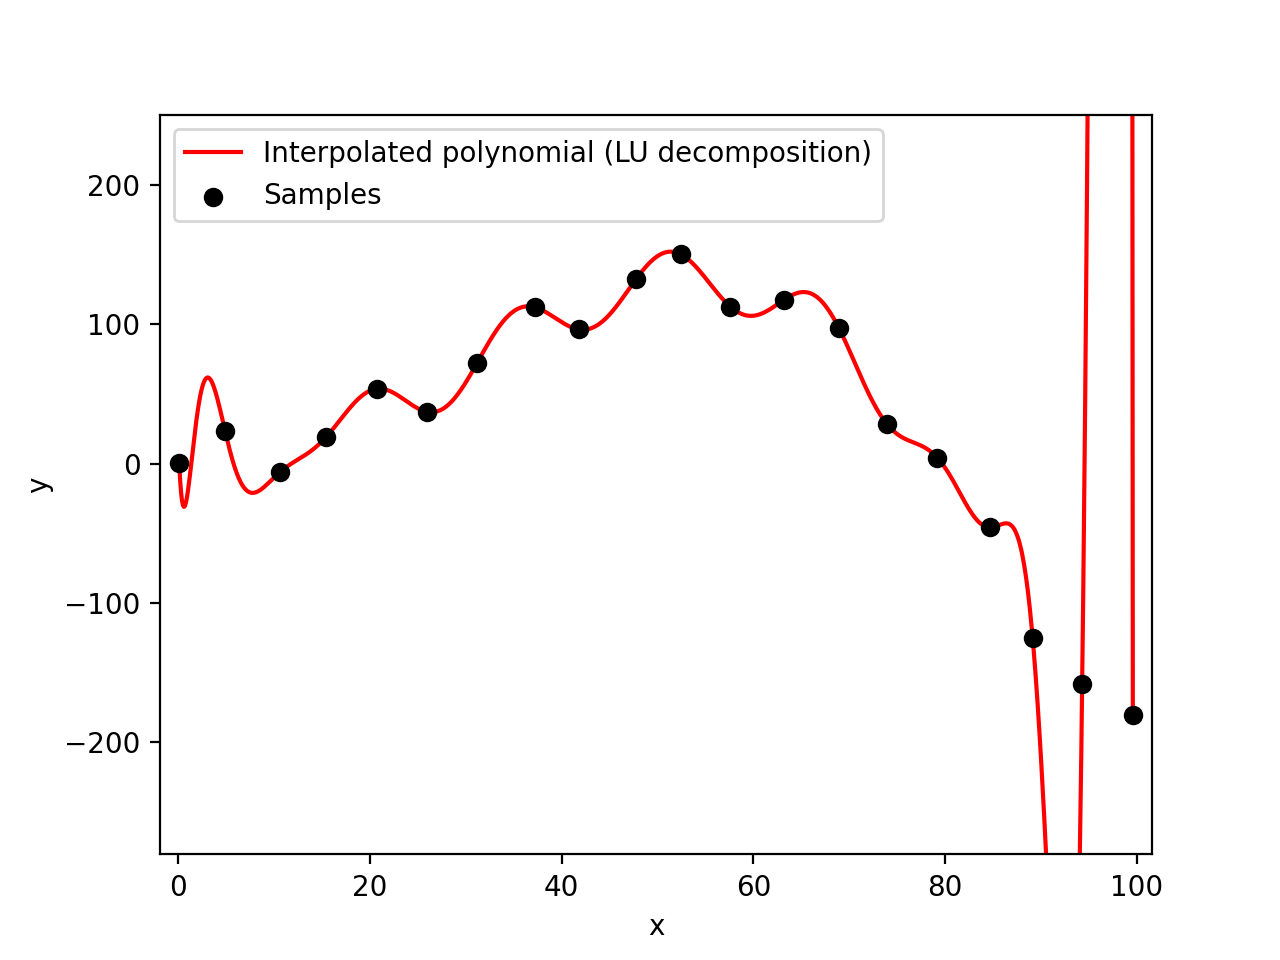
\includegraphics[width=0.9\linewidth]{./plots/2A_LU_Decomposition_polynomial_fit.png}
  \caption{19th-degree polynomial that passes through all data points. Computed using LUD.}
  \label{fig:2A_interp}
\end{figure}

The absolute difference between the sample points and those calculated using Eq. 2 ($|y(x) - y_i|$) is so low that we can only see it if we plot in log scale. The error rises as we go to the end, which is expected from the large oscillations in the end, see Figure \ref{fig:2A_diff}.

\begin{figure}[h!]
  \centering
  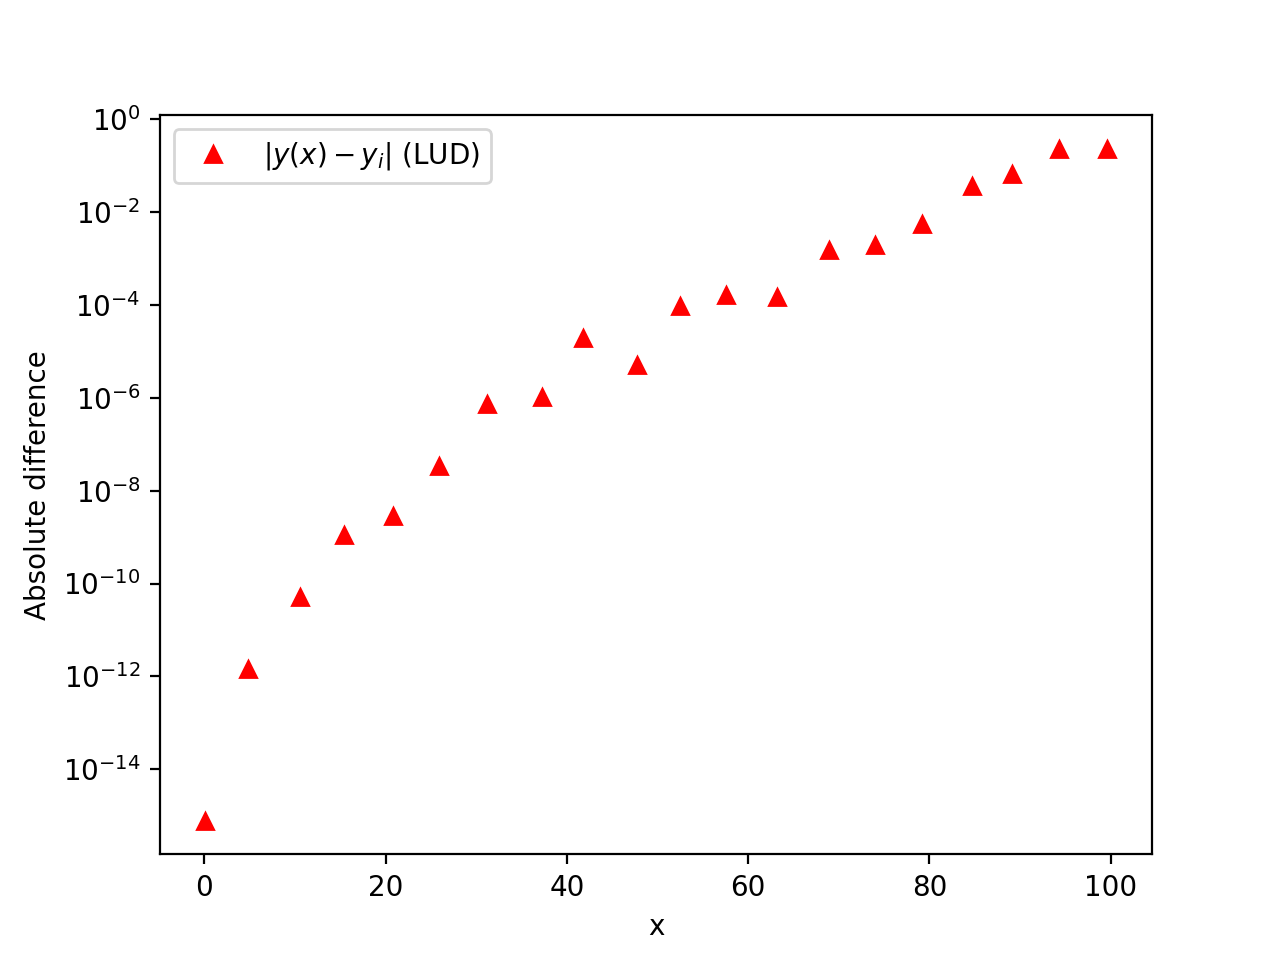
\includegraphics[width=0.9\linewidth]{./plots/2A_LU_Decomposition_absolute_difference.png}
  \caption{Absolute difference between $y(x)$ and $y_i$ as computed with LUD.}
  \label{fig:2A_diff}
\end{figure}

\subsection{2B}
Here, we apply Neville's algorithm to the same data. For Neville's algorithm, we first use a bisection algorithm to find the nearest sample points to x. This algorithm returns $j_{\rm{low}}$, the index of the lowest sample point in the interpolation, in which we make sure to not go beyond the edges of the dataset. Based on the order of the polynomial (in this case we want a 19th-degree polynomial), Neville's algorithm selects M tabulated points around x and sets the initial $P_i$ values at those $y$ values. We update the $P_i$ values using the equation for $H(x)$. In the end, $P_0$ holds the solution, with which we can create the interpolated polynomial. The polynomial is (as expected) the same as the one created with LUD, see Figure \ref{fig:2B_interp} with very slight differences in the error, as can be seen in Figure \ref{fig:2B_diff}.

\begin{figure}[h!]
  \centering
  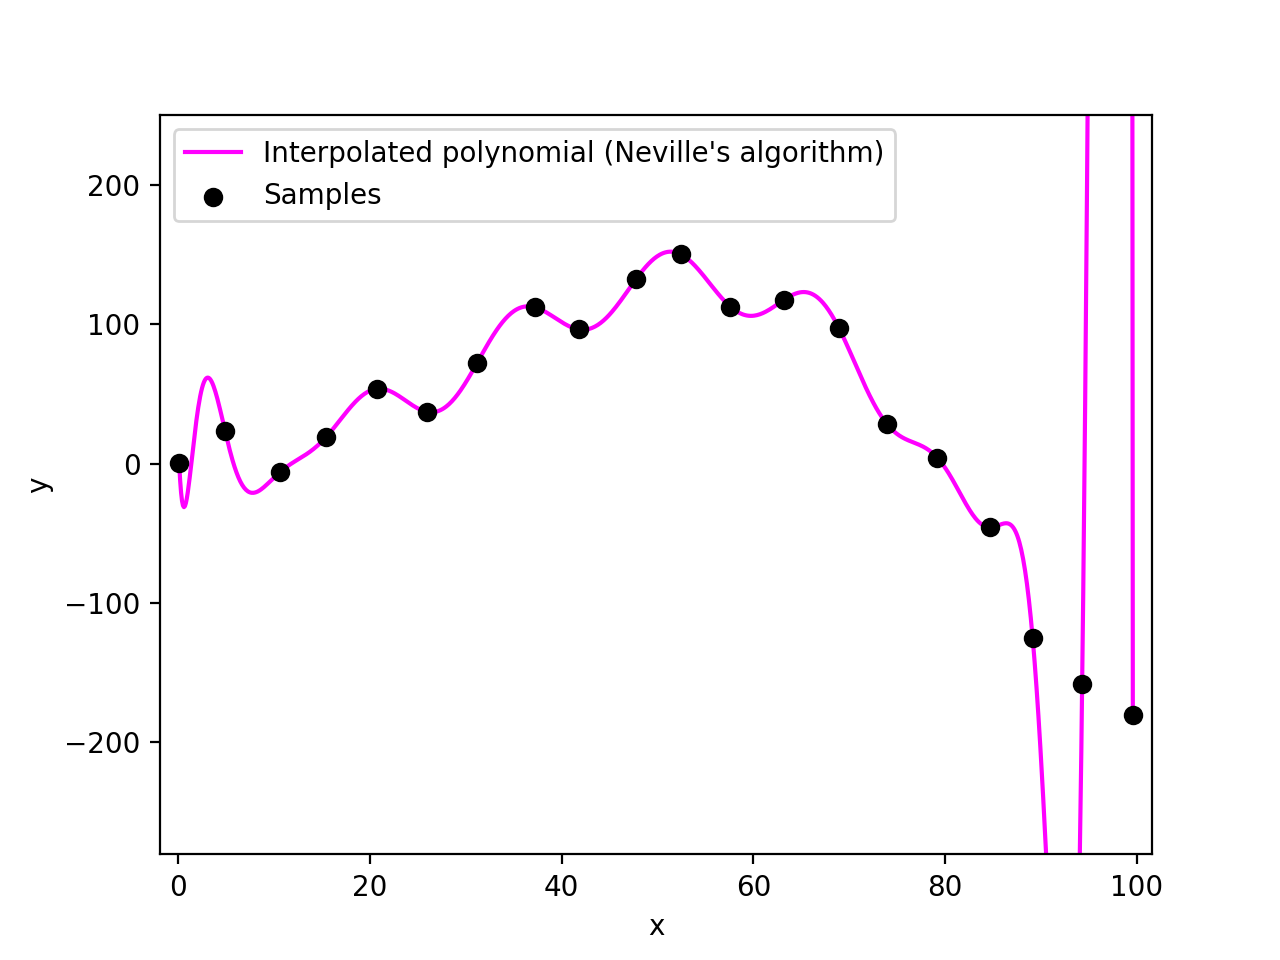
\includegraphics[width=0.9\linewidth]{./plots/2B_Neville_interpolation.png}
  \caption{19th-degree polynomial that passes through all data points. Computed using Neville's Algorithm.}
  \label{fig:2B_interp}
\end{figure}

\begin{figure}[h!]
  \centering
  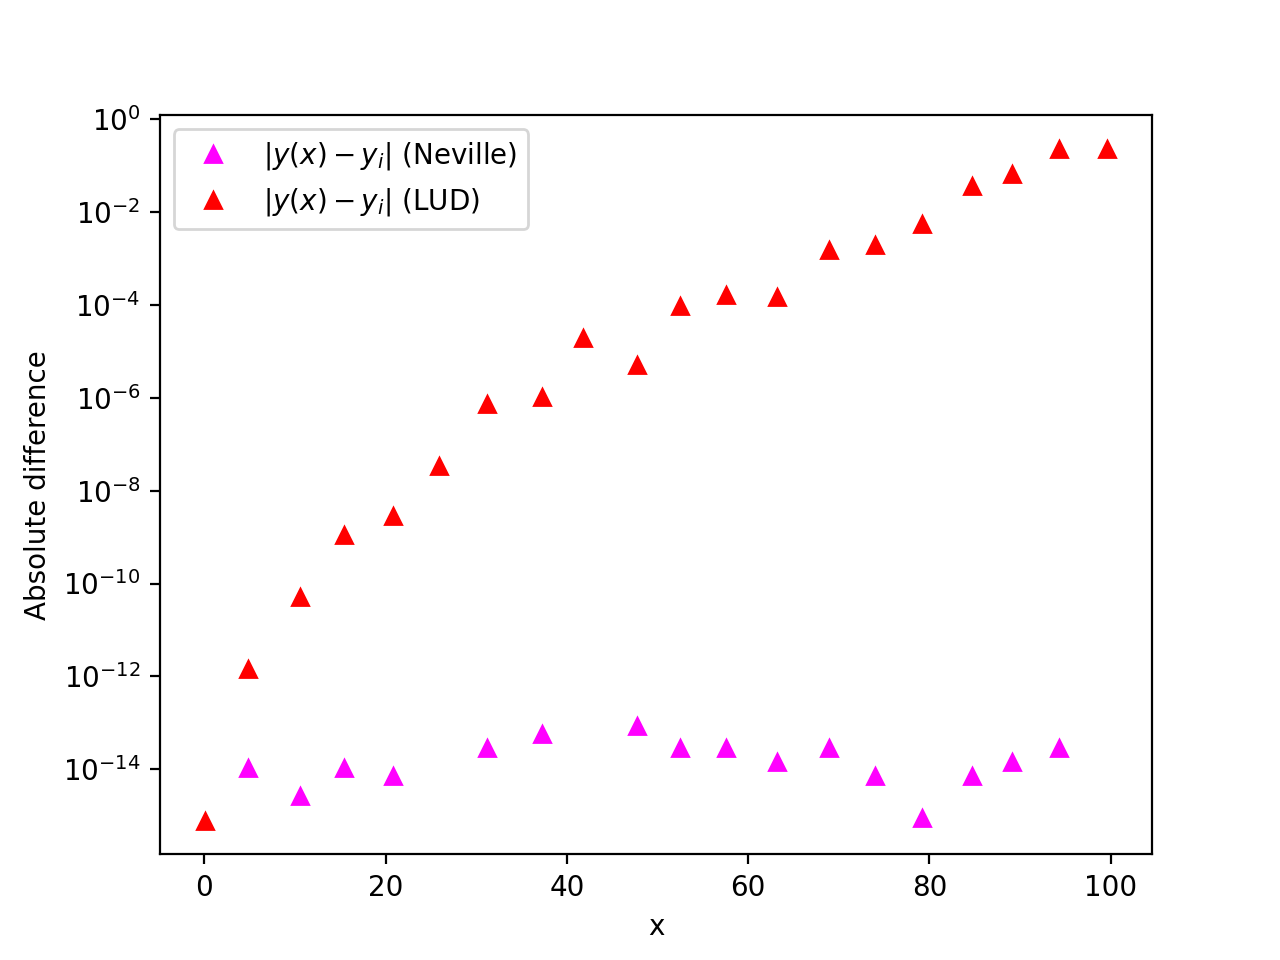
\includegraphics[width=0.9\linewidth]{./plots/2B_AbsoluteDiff_LU_Neville.png}
  \caption{Absolute difference between $y(x)$ and $y_i$ as computed with Neville's Algorithm. Compared with the absolute difference of LUD}
  \label{fig:2B_diff}
\end{figure}

\subsection{2C}
We can also interate on LUD to possibly lower the error. For that, we use the following:
\begin{equation}
    Ax' = b
\end{equation}
\begin{equation}
    \delta_b = Ax' - b
\end{equation}
and also,
\begin{equation}
    A\delta_x = \delta_b
\end{equation}
and,
\begin{equation}
    \delta_x = LU(A,\delta_b)
\end{equation}
and,
\begin{equation}
    x' = LU(A,b)
\end{equation}
so,
\begin{equation}
    x'' = x' - \delta_x = LU(A,b) - LU(Ax' - b).
\end{equation}

To calculate $Ax'$ we wrote a function for matrix multiplication. We then computed 10 LUD iterations, which gave a visually identical polynomial to the single-iteration LUD and Neville's algorithm, as seen in Figure \ref{fig:2C_interp}.

\begin{figure}[h!]
  \centering
  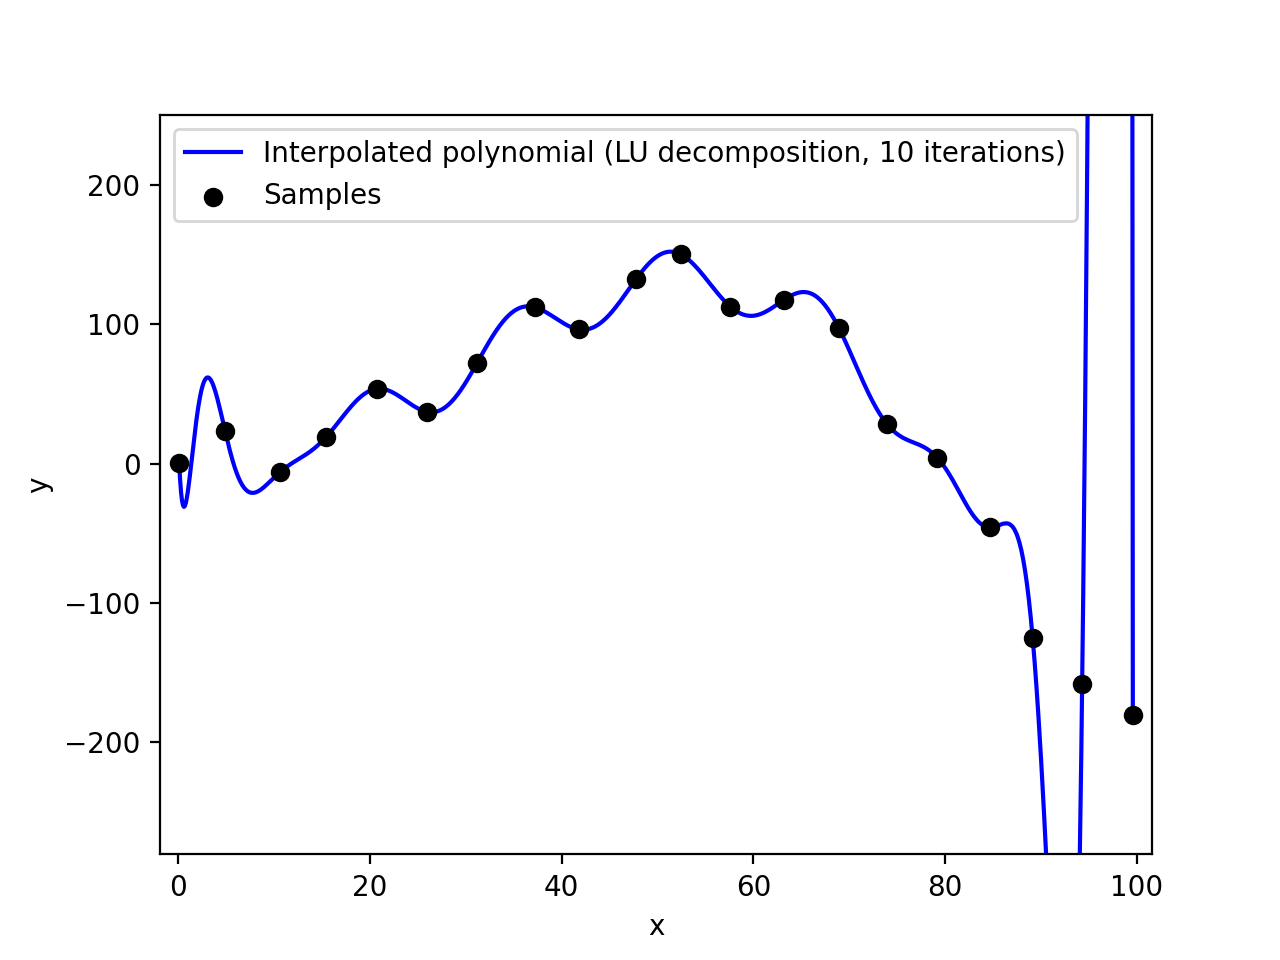
\includegraphics[width=0.9\linewidth]{./plots/2C_LU_Decomposition_iterative_polynomial_fit.png}
  \caption{19th-degree polynomial that passes through all data points. Computed using iterative LUD.}
  \label{fig:2C_interp}
\end{figure}

The absolute differences of the single-iteration LUD and iterative LUD differ only very slightly, so we conclude that our LUD algorithm was already optimized for 1 iteration, see Figure \ref{fig:2C_diff}.

\begin{figure}[h!]
  \centering
  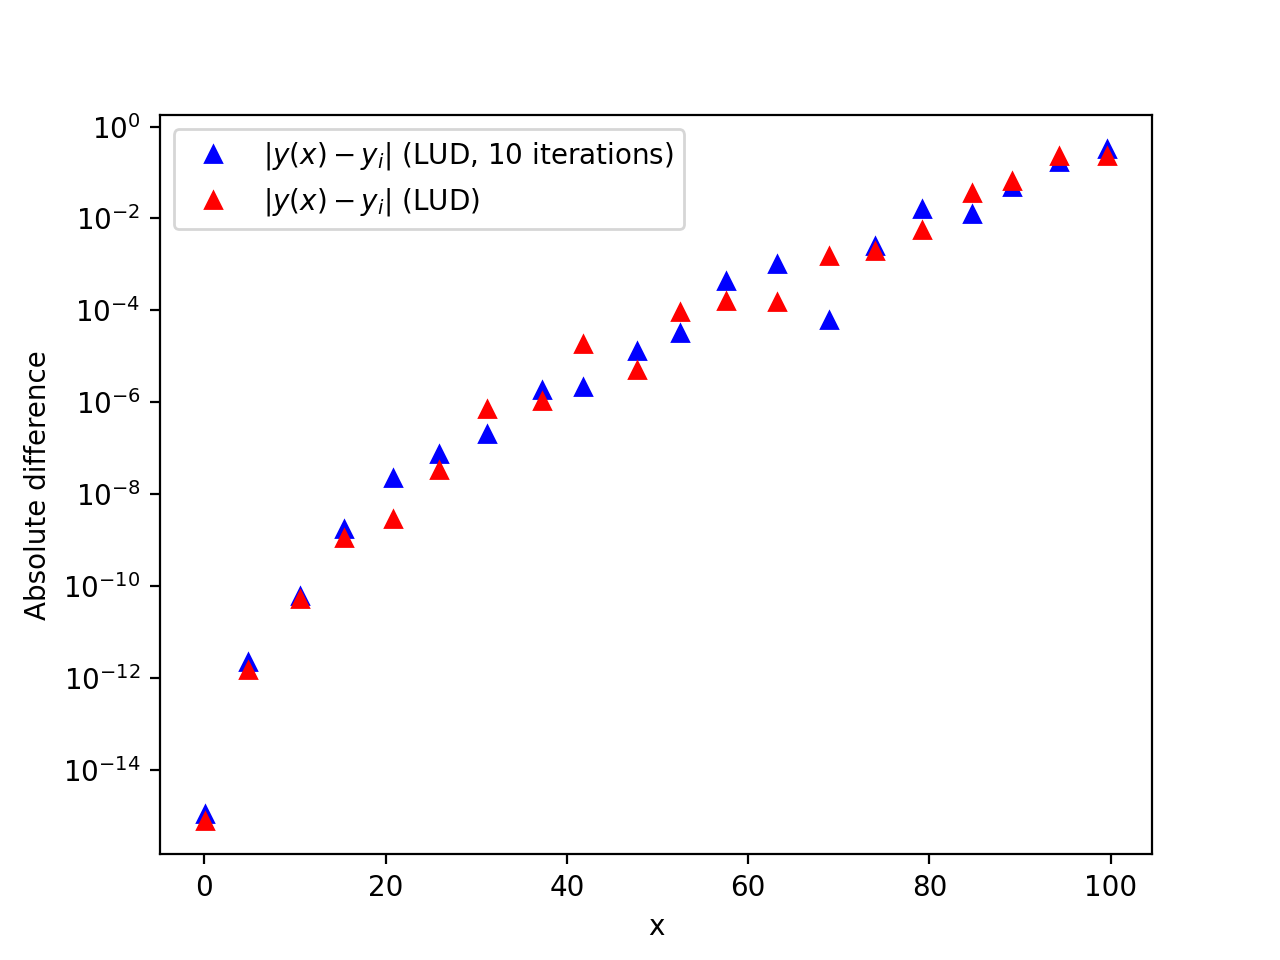
\includegraphics[width=0.9\linewidth]{./plots/2C_AbsoluteDiff_LU_iterative.png}
  \caption{Absolute difference between $y(x)$ and $y_i$ as computed with iterative LUD. Compared with the absolute difference of single-iteration LUD}
  \label{fig:2C_diff}
\end{figure}

\subsection{2D}
The time results for 2A, 2A and 2C can be found in the text output below the code. single-iteration LUD is the fastest, with iterative LUD in close second (which is expected since we have to do more operations with the matrix multiplication), and Neville's in third. Neville being the slowest is also expected, as the order of operations done is significantly higher for Neville's Algorithm compared to LUD, so it is not strange that LUD is the most efficient.


See the code below for our implementation of this exercise:
\lstinputlisting{NUR_Handin_1_2.py}

See the text below for the output of the code:
\lstinputlisting{NUR_Handin_1_2_output.txt}